\documentclass[times, utf8, seminar, numeric]{fer}

\usepackage{booktabs}
\usepackage{hyperref}
\usepackage{enumitem}
\usepackage{mathtools}
\usepackage{listings}
\usepackage{multirow}
\usepackage{tikz}
\usepackage{svg}
\usepackage{listings}
\usepackage[croatian,boxed,noline]{algorithm2e}
\usepackage[group-separator={,}]{siunitx}
\SetKwProg{Fn}{Funkcija}{}{}

\definecolor{dkgreen}{rgb}{0,0.6,0}
\definecolor{gray}{rgb}{0.5,0.5,0.5}
\definecolor{mauve}{rgb}{0.58,0,0.82}

% ovo su postavke za kod
\lstset{frame=tb,
  language=Python,
  aboveskip=3mm,
  belowskip=3mm,
  showstringspaces=false,
  columns=flexible,
  basicstyle={\small\ttfamily},
  numbers=left,
  numberstyle=\tiny\color{gray},
  keywordstyle=\color{blue},
  commentstyle=\color{dkgreen},
  stringstyle=\color{mauve},
  breaklines=true,
  breakatwhitespace=true,
  tabsize=3
}

\renewcommand{\lstlistingname}{Isječak koda}% Listing -> Isječak koda
\newcommand{\specialcell}[2][c]{\begin{tabular}[#1]{@{}c@{}}#2\end{tabular}}

\begin{document}

\title{Izgradnja binarnog stabla valića kao RRR strukture}
\author{Mislav Magerl, Matija Milišić, Mateo Šimonović}
\voditelj{doc. dr. sc. Mirjana Domazet-Lošo}

\maketitle

\tableofcontents

\chapter{Uvod}
U ovom radu opisana je implementacija stabla valića\citep{alexbowe}  koje se koristi za brze $rank$ i $select$ upite nad ulaznim nizom znakova. Konkretna implementacija bazirana je na RRR strukturi \citep{DBLP:journals/corr/abs-0705-0552}.



Brza implementacija metoda $rank$ i $select$ znače da se stablo valića može iskoristiti za pronalaženje podudarajućih nizova, odnosno podnizova. 

U poglavlju \ref{sec:rrr} opisana je RRR struktura i dan je primjer upita koji se nad tom strukturom mogu zvati. U poglavlju \ref{sec:wavelet-tree} opisano je stablo valića te je također dan primjer upita koji se nad tom strukturom mogu zvati. U poglavlju \ref{sec:results} napisana su mjerenja koja su pokrenuta nad sintetičkim ulazima te nad stvarnim ulazima koji predstavljaju genome nekih virusa, bakterija i organizama. Također napravljena je usporedba s implementacijom studenata s kolegija Bioinformatika akademske godine 2015/2016. U poglavlju \ref{sec:implementation} opisani su neki detalji implementacije projekta u jeziku C++.

U zadnjem \ref{sec:conclusion}. poglavlju dan je kratki zaključak o implementaciji i rezultatima ispitivanja rješenja te je dano nekoliko primjera gdje bi se, u budućnosti, mogla napraviti poboljšanja u odnosu na ovu implementaciju. 

\chapter{RRR struktura}
\label{sec:rrr}
RRR struktura je podatkovna struktura koja se koristi za brze rank, select te access upite nad binarnim nizom znakova. RRR strukturu su predložili Raman, Raman and Rao \citep{DBLP:journals/corr/abs-0705-0552} te je po njima i dobila ime. Metoda $rank(i)$ odgovara na pitanje koliko se jedinica nalazi u ulaznom nizu do, uključivo, indeksa $i$. Metoda $select(i)$ odgovara na pitanje na kojem se indeksu u ulaznom nizu nalazi $i$-ta jedinica. Metoda $access(i)$ odgovara koji znak se nalazi na indeksu $i$ u ulaznom nizu - nula ili jedinica.

\section{Izgradnja strukture}
\label{sec:izgradnja-rrr}
Ulazni binarni niz podijeljen je u blokove, a blokovi su podijeljeni u superblokove. Broj znakova u bloku ($b$) te broj blokova u superbloku ($f$) su parametri strukture. Na slici \ref{fig:rrr} prikazan je primjer RRR strukture s parametrima $b=5$ te $f=2$. Ako nisu eksplicitno zadani, parametri se računaju u ovisnosti o veličini ulaznog niza ($n$):
$b=\frac{\log_2n}{2}$,
$f=2  \log_2n$.
Svaki blok struktura pamti par vrijednosti - klasu \engl{class} - $c$ i pomak \engl{offset} - $o$. Klasa je broj jedinica u bloku, a pomak je indeks permutacije jedinica u lookup tablici koja je zadjednička za cijelu strukturu. 

\textbf{Lookup tablica}

Lookup tablica sadrži $2^b$ redova. Svaki red prikazuje jednu od mogućih različitih blokova veličine $b$ - sve kombinacije nula i jedinica u nizu veličine $b$. Dodatno, tablica je na taj način izgrađena da su prvo sve permutacije s nula jedinica, zatim sve permutacije s jednom, dvije te naposlijetku $b$ jedinica. Za svaki zapis zapisan je niz kumulativne sume do $i$-tog elementa u tom bloku. Dio lookup tablice prikazan je na slici \ref{fig:lookup}. Vremenska složenost izgradnje lookup tablice je $O(b \cdot 2^b)$, odnosno izraženo preko veličine ulaznog niza $O(n \cdot \log_2n)$. Memorijska složenost je također $O(b \cdot 2^b)$.

\textbf{Izgradnja strukture}

Nakon izgradnje lookup tablice za svaki blok se računa klasa i pomak te se spremaju u strukturi umjesto originalnog niza. Jedan zapis o klasi veličine je 1B iz razloga što je ukupan broj klasa $log_2b$ što za vrijednosti $b$ do $16$, odnosno vrijednosti $n$ do $10^{10}$, iznosi $4$ bita. Jedan zapis o pomaku je veličine 2B iz razloga što za svaku klasu $c$ ima $\binom{b}{c}$ zapisa, tj. maksimalno $\binom{b}{\frac{b}{2}}$. Ako se uzme da je $n$ maksimalno $10^{10}$, $b$ iznosi maksimalno $16$. Najveći pomak u nekoj klasi tada iznosi $\binom{16}{8}=12870$ za što nije potrebno više od 2B.  Ukupno se, dakle, za jedan blok troši 3B memorije. Ukupna memorijska složenost je $O(\frac{n}{b})$, odnosno izraženo samo preko veličine niza $O(\frac{n}{log_2n})$
Također, struktura pamti i kumulativnu sumu do svakog superbloka. Memorijska složenost te sume je $O(frac{n}{b f})$, odnosno izraženo samo preko veličine niza $O(\frac{n}{(\log_2n)^2})$.

\begin{figure}[ht]
	\centering
	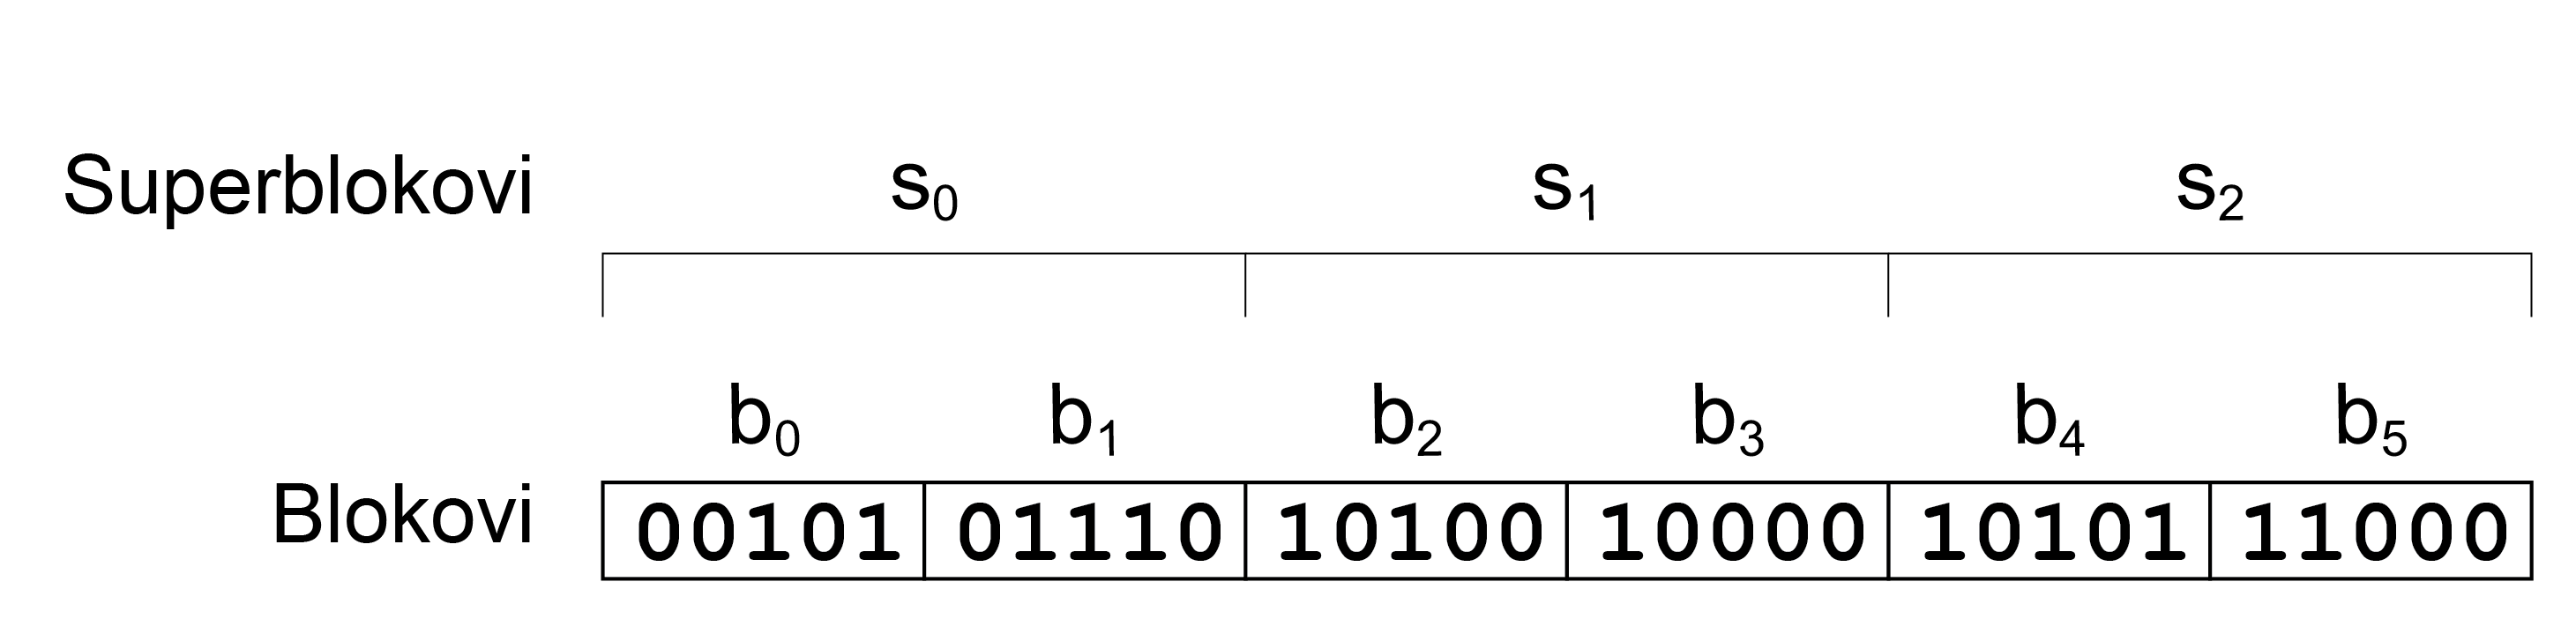
\includegraphics[width=15cm]{img/rrr_blocks.png}
	\caption{Prikaz blokova i superblokova RRR strukture}
	\label{fig:rrr}
\end{figure}

\begin{figure}[ht]
	\centering
	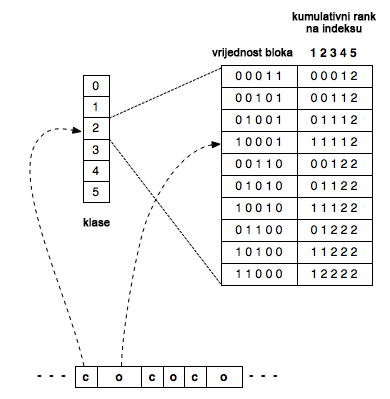
\includegraphics[width=10cm]{img/rrr-binary-table.png}
	\caption{Prikaz lookup tablice unutar RRR strukture}
	\label{fig:lookup}
\end{figure}


\section{Operacije nad strukturom}
U sljedećim odlomcima bit će opisane implementacije operacija $rank$, $select$ i $access$ nad RRR strukturom.


\subsection{Rank}
U RRR strukturi postoje dvije rank operacije - $rank_0(i)$ te $rank_1(i)$. Operacija $rank_0(i)$ vraća broj nula do, uključivo, indeksa $i$, a $rank_1(i)$ broj jedinica do indeksa. 
Jedna metoda može se vrlo jednostavno izraziti pomoću druge. Tako implementacija metode $rank_0(i)$ izgleda ovako:


\begin{algorithm}[H]
 \caption{Pseudokod metode $rank_0$}
 \Fn{\texttt{rank0(i)}}{
	\Vrati \texttt{i + 1 - rank1(i)}\;

 }
\end{algorithm}


Operacija $rank_1(i)$ se računa na sljedeći način:
\begin{enumerate}
	\item Izračuna se indeks superbloka te bloka u kojem se pozicija $i$ nalazi
	\item Izračuna se suma svih blokova do bloka u kojem se pozicija $i$ nalazi
	\item Pomoću lookup tablice se na sumu dodaje suma brojeva do pozicije $i$
\end{enumerate}
Pseudokod:

\begin{algorithm}[H]
 \caption{Pseudokod metode $rank_1$}
 \Fn{\texttt{rank1(i)}}{
 	\texttt{indexBloka = i / b\;
	indexSuperbloka = i / (b*f)\;
	rez = kumulativnaSumaSuperbloka(indexSuperbloka - 1)\;
	\Za {\texttt{i = indexSuperbloka * f .. indexBloka}}{
		rez += klasa[i]\;
	}
	c = klasa[indexBloka]\;
	o = pomak[indexBloka]\;
	rez += lookup[c][o][index - indexBloka * b]\;
	\Vrati rez;}

 }
\end{algorithm}

Složenost rank operacija je $O(f)$, odnosno $O(log_2n)$.

\textbf{Primjer izvođenja operacije $rank_1$}:

Tražimo na primjeru slike \ref{fig:rrr} $rank_1(25)$. Ulazni niz, blokovi i superblokovi su 0-indeksirani. Parametri RRR-a su $b=5$ i $f=2$. U prvom koraku računamo $indexBloka=\frac{25}{5}=5$.  U sljedećem računamo $indexSuperbloka=\frac{25}{5 \cdot 2}=2$ (ovdje koristimo cjelobrojnu aritmetiku). U variablu $rez$ dodajemo kumulativnu sumu do superbloka $1$. Ona iznosi $8$. Zatim u petlji s varijablom $i$ idemo od $indexSuperbloka \cdot f=4$ do $indexBloka=5$, isključivo. U toj petlji idemo samo s $i=4$ te u varijablu $rez$ dodajemo klasu četvrtog bloka koja iznosi $3$. Sada je vrijednost varijable $rez$ jednaka $11$. Naposlijetku čitamo klasu i indeks traženog bloka koje iznose: $c=2$, $o=9$. Dodajemo $rez+=lookup[2][9][25-5*5]$, što možemo sa slike \ref{fig:lookup} iščitati da iznosi $1$. Konačna vrijednost u operacija $rank_1$ vraća je 12. 


\subsection{Select}
Kao i za rank operaciju i select operacija ima svoje dvije varijante - $select_0(i)$ te $select_1(i)$ koje vraćaju indeks $i$-tog pojavljivanja nule odnosno jedinice. Te dvije metode mogu se napisati općenito, jednom funkcijom koja kao parametar prima boolean parametar koji određure traži zove li se $select_0$ ili $select_1$.
Operacija $select_1(i)$ računa se na sljedeći način:
\begin{enumerate}
	\item Pronađi binarnim pretraživanjem superblok u kojem se nalazi tražena jedinica
	\item U brojač pohrani sumu jedinica do prethodnog superbloka
	\item Dodaj u brojač blokove sve dok ne dođeš do bloka koji prethodi bloku u kojem je tražena jedinica
	\item Binarnim pretraživanjem pronađi poziciju tražene jedinice u bloku.
\end{enumerate}
Pseudokod:

\begin{algorithm}[H]
 \caption{Pseudokod metode $select$}
 \Fn{\texttt{select(i, tip)}}{
 	\texttt{indexSuperbloka = pronađiSuperblok(i, tip)\;
	brojač = kumulativnaSumaSuperbloka(indexSuperbloka - 1, tip)\;
	indexBloka = indexSuperbloka * f\;
	\Dok{\texttt{brojač < i}}{
		brojač = brojač + dohvatiKlasuBloka(indexBloka, tip)\;
		indexBloka = indexBloka + 1\;
	}
	indexBloka = indexBloka - 1\;
	brojač = brojač - dohvatiKlasuBloka(indexBloka, tip)\;
	indexUBloku = pronađiIndeksUBloku(i - brojač, tip)\;
 	\Vrati indexBloka * b + indexUBloku\;
 	}

 }
\end{algorithm}

Metode \texttt{pronađiSuperblok}, \texttt{kumulativnaSumaSuperbloka}, \texttt{dohvatiKlasuBloka} i \texttt{pronađiIndeksUBloku} primaju kao parametar \texttt{tip}. Varijabla \texttt{tip} je istinita ako se traži jedinica, odnosno lažna ako se traži nula. Ovisno o tom parametru se metode i ponašaju. Metode \texttt{pronađiSuperblok} i \texttt{pronađiIndeksUBloku} rade binarno pretraživanje kako bi pronašle indekse.
Složenost možemo rastaviti na nekoliko dijelova. Vremenska složenost traženja superbloka je $O(\frac{n}{b \dot f})$, tj. $O(\frac{n}{(\log_2n)^2})$. Zatim se traži indeks bloka unutar superbloka - $O(f)$, tj. $O(\log_2n)$. Složenost dohvaćanja klase je konstantna, $O(1)$. Složenost traženja indeksa u bloku je $O(\log_2b)$, odnosno $O(\log_2(\log_2n))$.

\textbf{Primjer izvođenja operacije $select_1$}:

Tražimo na primjeru slike \ref{fig:rrr} $select_1(12)$. Primjetimo da bi rezultat trebao biti $25$ jer je $rank_1(25)=12$. Ulazni niz, blokovi i superblokovi su 0-indeksirani. Parametri RRR-a su $b=5$ i $f=2$. U prvom koraku binarno pretražujemo superblok u kojem se nalazi dvanaesta jedinica. Dobivamo $indexSuperbloka=2$. U varijablu $broja\check{c}$ spremamo kumulativnu sumu do superbloka s indeksom $1$ - $broja\check{c}=8$. Varijabla $indexBloka=2 \cdot 2=4$. U \textit{dok} petlji se brojač poveća na vrijednost $11$, zatim na vrijednost $13$. Uz brojač, varijabla $indexBloka$ se poveća najprije na $5$ pa na $6$. Na izlasku iz petlje, $indexBloka$ i $broja\check{c}$ se pomiću ulijevo. Sada je $indexBloka=5$, a $broja\check{c}=11$. Metoda $pronađiIndeksUBloku(12-11)$ radi binarno pretraživanje nad lookup tablicom i vraća vijednost $indexUBloku=0$. Konačno, funkcija vraća vijednost $5 \cdot 5 + 0=25$.

\subsection{Access}
Metoda $access(i)$ vraća koji se znak nalazi na danoj poziciji - nula ili jedan. Metoda je vrlo jednostavna. Jednostavno se računa razlika između $rank1$ od trenutne pozicije i prethodne pozicije.

\begin{algorithm}[H]
 \caption{Pseudokod metode $access$}
 \Fn{\texttt{access(i)}}{
 	\texttt{\uAko{i==0}{
		\Vrati rank1(i)\;
 	} \Inace{
		\Vrati rank1(i) - rank1(i - 1)\;
 	}
 	}

 }
\end{algorithm}


\textbf{Primjer izvođenja operacije $access$}:

Tražimo na primjeru slike \ref{fig:rrr} $access_1(25)$. Ulazni niz, blokovi i superblokovi su 0-indeksirani. Parametri RRR-a su $b=5$ i $f=2$. Rezultat je $rank_1(25)-rank_1(24)$ što je jednako $1$.

\chapter{Stablo valića}
\label{sec:wavelet-tree}
Stablo valića \engl{Wavelet Tree} je struktura podataka koja omogućava efikasno spremanje niza znakova nad proizvoljnom abecedom u memoriji računala i efikasnog odgovaranja na određena pitanja nad istim. Iako originalno predstavljeno od tvoraca strukture Grossija, Gupte i Vittera \citep{Grossi:2003:HET:644108.644250} za rad isključivo nad nizovima, stablo valića se pokazalo kao vrlo efikasna struktura podataka za predstavljanje permutacija i rešetke točaka i pronašlo je primjenu u raznim područjima, od obrade i indeksiranja teksta, do teorije grafova i geometrije. \citep{navarro-wavelet-trees-for-all}

Stablo valića je podatkovna struktura koja ulazni niz znakova kodira kao stablo binarnih nizova. Na taj je način ostvarena sažeta struktura podataka \engl{succinct data structure}, odnosno to je struktura podataka koja koristi memorije blisko donjoj granici definiranoj teorijom informacije (konkretno, $N + o(N)$ bitova memorije gdje je $N$ teorijski optimum za pohranu podataka), a i dalje nudi efikasnu implementaciju odgovora na razne upite o sadržanim podacima.


\begin{figure}[ht]
	\centering
	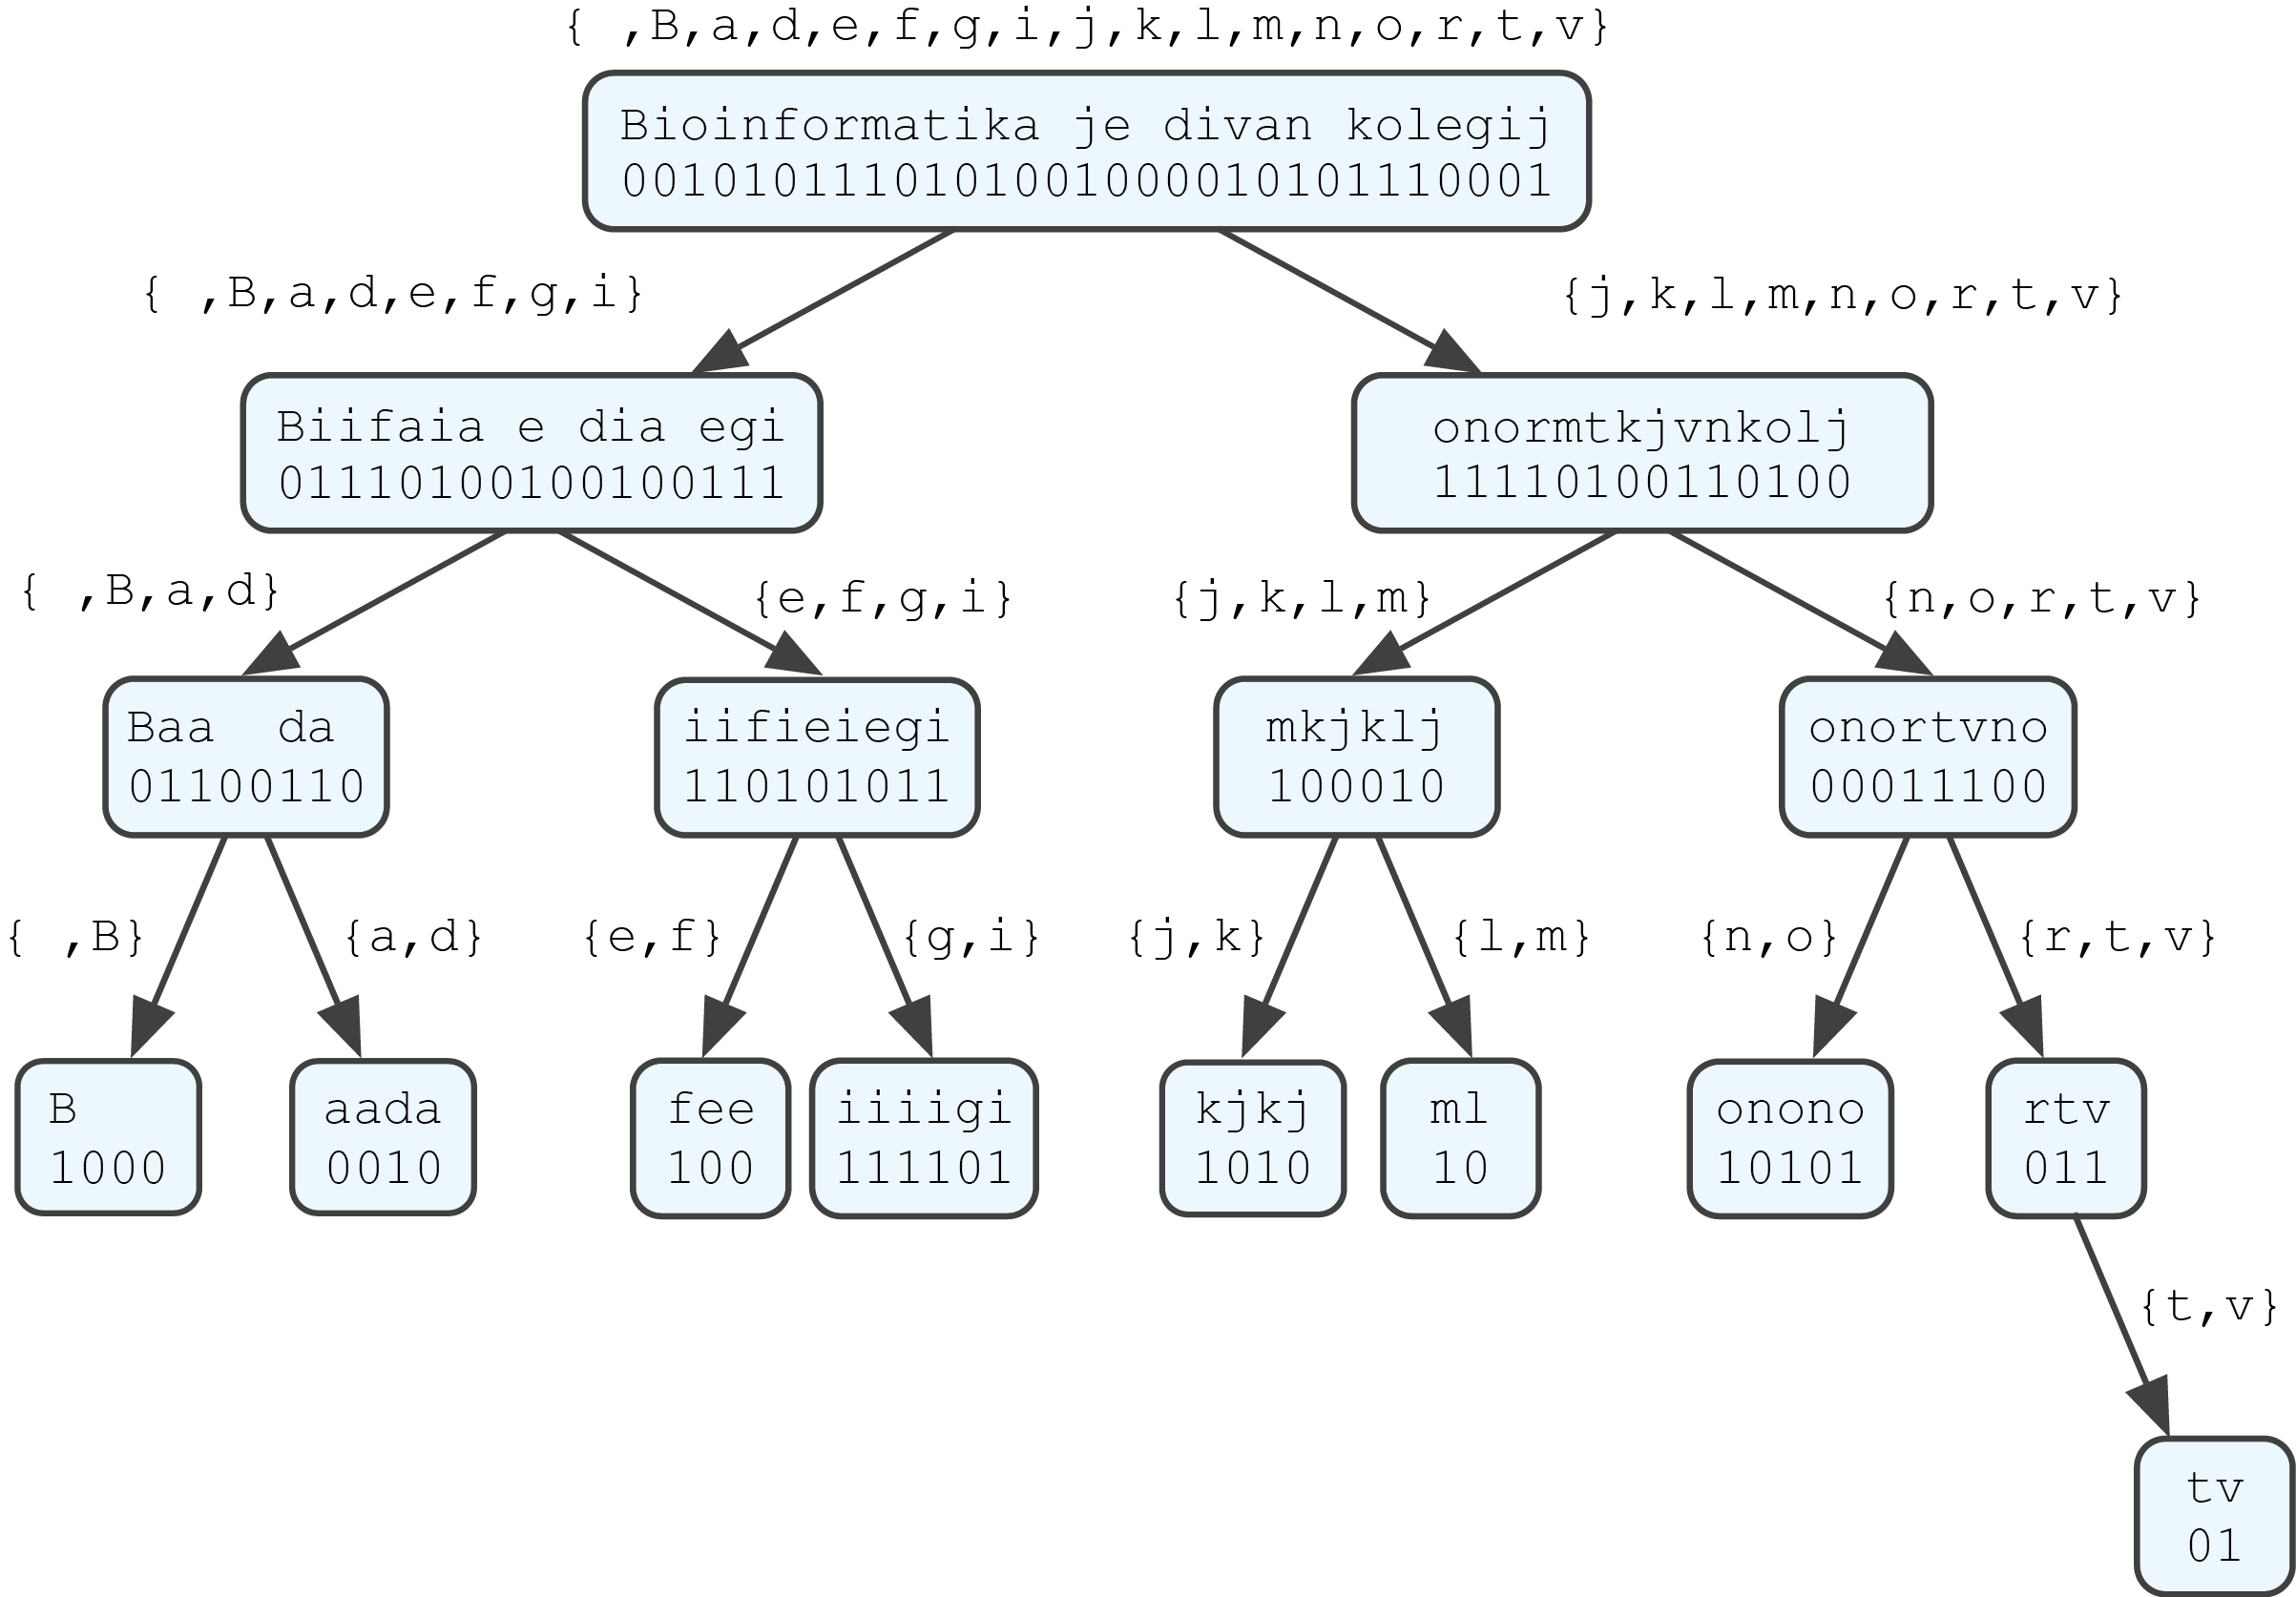
\includegraphics[width=\textwidth]{img/wavelet_tree_example.png}
	\caption{Stablo valića za ulazni niz "Bioinformatika je divan kolegij"}
	\label{fig:wavelet-tree-example}
\end{figure}


Na slici \ref{fig:wavelet-tree-example} prikazan je primjer izgrađenog stabla valića za ulazni niz znakova “Bioinformatika je divan kolegij”. Stablo je binarno i balansirano, a gradi se rekurzivnim postupkom počevši od korijena stabla koji predstavlja cijeli ulazni niz pa do listova koji predstavljaju jedinstveno označene znakove. U poglavlju \ref{sec:izgradnja-stabla} detaljnije je opisan postupak izgradnje stabla na danom primjeru. U praksi postoje dvije moguće implementacije izgradnje stabla valića: prva koja gradi stablo dok svako slovo u ulaznoj abecedi ne postane list s jedinstvenim binarnim kodom, a druga koja gradnju stabla zaustavi kada čvor sadrži samo dva različita znaka jer ih je tada binarnim nizom već moguće razlikovati. U ovom je radu korištena druga implementacija radi uštede memorije zbog nepotrebnog spremanja dodatne dubine stabla. Važno je primjetiti da o duljini ulaznog niza ovisi duljina vektora bitova u svakom čvoru stabla, dok dubina stabla ovisi samo o veličini abecede ulaznog niza. Također, bitno je napomenuti da su znakovi u čvorovima prikazani radi razumijevanja postupka izgradnje stabla, ali se u strukturi ne pamte. Stablo valića omogućuje efikasnu implementaciju operacija koje se u literaturi pojavljuju kao rank, select i access, a njihova važnost i implementacijski detalji objašnjeni su u poglavlju \ref{sec:operacije-nad-stablom}.

\section{Izgradnja stabla}
\label{sec:izgradnja-stabla}

Stablo valića gradi se rekurzivnim postupkom koji kreće od niza znakova $\mathnormal{S} = s_1s_2 \dots s_n$, uz $s_i \in \Sigma$, gdje je $\Sigma$ abeceda \engl{alphabet} ulaznog niza znakova. \citep{navarro-wavelet-trees-for-all} Pseudokod algoritma za izgradnju stabla valića prikazan je u nastavku. Algoritam kreće od korijena stabla i rekurzivno se spušta do listova.

\begin{algorithm}[H]
 \caption{Izgradnja stabla valića}
 \Fn{\texttt{izgradiStabloValića($\mathnormal{S}$, $\Sigma$)}}{
 	\Ako{$|\Sigma|\leqslant2$}{
		\Vrati\;
 	} 
 	$\Sigma_1$, $\Sigma_2 \leftarrow$  podijeliNaDvaJednakaDijela($\Sigma$)\;
 	pridijeli svim znakovima $s_i \in \mathnormal{S}$ kod $0$ \textbf{ako} $s_i \in \Sigma_1$, \textbf{inače} kod $1$\;
 	$\mathnormal{S}_1$, $\mathnormal{S}_2 \leftarrow$  grupiraj znakove iz $\mathnormal{S}$ prema kodu\;
	izgradiStabloValica($\mathnormal{S}_1$, $\Sigma_1$)\;
	izgradiStabloValica($\mathnormal{S}_2$, $\Sigma_2$)\;
 }
\end{algorithm}

U nastavku slijedi opis izgradnje stabla za primjer sa slike \ref{fig:wavelet-tree-example}.
Na samom početku, ulazni niz znakova je $ \mathnormal{S} = Bioinformatika\ je\ divan\  kolegij $. Abeceda niza $\mathnormal{S}$ je
 $$ \Sigma = \{\ ,B,a,d,e,f,g,i,j,k,l,m,n,o,r,t,v\} $$. 
 Pritom je duljina ulaznog niza znakova $ |\mathnormal{S}| =  31 $ znak, a veličina abecede $ |\Sigma| = 17 $ znakova. Znakovi abecede su poredani uzlazno prema ASCII kodu. 

Zatim se abeceda $\Sigma$ dijeli na dva približno jednaka dijela $ \Sigma_1 = \{ ,B,a,d,e,f,g,i\} $ i $ \Sigma_2 = \{j,k,l,m,n,o,r,t,v\} $. Sljedeći je korak kodirati ulazni niz znakova $\mathnormal{S}$ na način da se svakom znaku ulaznog niza $s_i$ pridijeli kod $0$ ako je $ s_i \in \Sigma_1$, te kod $1$ ako je $ s_i \in \Sigma_2 $. Rezultat ove operacije je sljedeći binarni niz $ 0010101110101001000010101110001 $. 

Na osnovi dobivenog binarnog niza stvaraju se nizovi znakova $\mathnormal{S}_1$ i $\mathnormal{S}_2$ tako da se znakovi kodirani kodom $0$ izdvoje u niz $\mathnormal{S}_1$, a znakovi kodirani kodom $1$ u niz $\mathnormal{S}_2$. Na ovom su primjeru na taj način dobiveni sljedeći nizovi $\mathnormal{S}_1 = Biifaia\ e\ dia\ egi$ te $\mathnormal{S}_2 = onormtkjvnkolj$. S tim se nizovima, zajedno s odgovarajućim abecedama $\Sigma_1$ i $\Sigma_2$, postupak ponavlja za lijevo i desno dijete u stablu.

Poseban je slučaj kada postupak dolazi do lista i ne stvara novo dijete u stablu, a to se događa kada je $|\Sigma| <= 2$. Razlog zbog kojeg nije potrebno stvarati nove čvorove u stablu u tom slučaju je zbog toga što se svaki znak ulaznog niza može jedinstveno kodirati samo s oznakama $0$ i $1$. Jedan od čvorova u stablu iz primjera sa slike \ref{fig:wavelet-tree-example} kod kojeg će se dogoditi taj poseban slučaj je čvor čiji je ulazni niz $\mathnormal{S} = aada$ te abeceda $ \Sigma = \{a,d\} $. Za promatrani čvor podijeli se abeceda na dva jednaka dijela i dobije $ \Sigma_1 = \{a\} $ i $ \Sigma_2 = \{d\} $ te se jednostavno čvoru pridružuje kodirani zapis $ \mathnormal{S}_{kod} = 0010 $ i ne generiraju djeca trenutnog čvora.

\section{Operacije nad stablom}
\label{sec:operacije-nad-stablom}

Stablo valića omogućava efikasno izvođenje tri osnovne operacije:

\begin{enumerate}
	\item $rank(i, c)$ - broj pojavljivanja znaka $c$ do uključivo $i$-te pozicije u ulaznom nizu znakova
	\item $select(i, c)$ - indeks $i$-tog znaka \textit{c} u ulaznom nizu znakova
	\item $access(i)$ - znak na $i$-toj poziciji u ulaznom nizu znakova
\end{enumerate}


U idućim poglavljima dani su opisi svake od navedenih operacija, njihov pseudokod te je pokazan primjer njihovog izvođenja nad stablom izgrađenim u poglavlju \ref{sec:izgradnja-stabla}.

\subsection{Rank}

\begin{algorithm}[H]
 \caption{Pseudokod $rank$ operacije nad stablom valića}
 \Fn{\texttt{rank($i$, $c$)}}{
  	\texttt{trenutniČvor = korijenStabla\;
	pozicija = i\;
	}
	
	\Dok{\texttt{trenutniČvor != NULL}}{
		\uAko{\texttt{$c \in $ trenutniČvor.desno}}{
			\texttt{pozicija = \texttt{rank1(pozicija)} - 1\;
			trenutniČvor = trenutniČvor.desno\;
			}
 		}
 		\Inace {
 			\texttt{pozicija = \texttt{rank0(pozicija)} - 1\;
 			trenutniČvor = trenutniČvor.lijevo\;
 			}
 		}
 		\Ako{\texttt{pozicija == -1}}{
			\textbf{izađi}\;
 		}
	}
	\Vrati \texttt{pozicija} + 1\;
}
\end{algorithm}

\subsection{Select}

\begin{algorithm}[H]
 \caption{Pseudokod $select$ operacije nad stablom valića}
 \Fn{\texttt{select($i$, $c$)}}{
	\texttt{trenutniČvor = čvorZaZnak($c$)\;
	pozicija = $i$\;
	}
	
	\uAko{\texttt{k\^{o}d(trenutniČvor) == 0}}{
		\texttt{pozicija = select0(pozicija)}\;
 	}
	\Inace {
 		\texttt{pozicija = select1(pozicija)}\;
 	}
	
	\Dok{\texttt{trenutniČvor != korijenStabla}}{
		\uAko{je \texttt{trenutniČvor} lijevo dijete}{
			\texttt{pozicija = trenutniČvor.roditelj.select0(pozicija+1)}\;
 		}
 		\Inace {
			\texttt{pozicija = trenutniČvor.roditelj.select1(pozicija+1)}\;
 		}
		\texttt{trenutniČvor = trenutniČvor.roditelj\;}
	}
	\Vrati \texttt{pozicija\;}
}
\end{algorithm}


\subsection{Access}

\begin{algorithm}[H]
 \caption{Pseudokod $access$ operacije nad stablom valića}
 \Fn{\texttt{access($i$)}}{
	\texttt{trenutniČvor = korijenStabla\;
	pozicija = $i$\;
	}
	
	\Dok{\texttt{trenutniČvor != NULL}}{
		\uAko{\texttt{access(pozicija)} == 0}{
			\texttt{pozicija = rank0(pozicija)\;
			\Ako{\texttt{trenutniČvor.lijevo == NULL}}{
				\Vrati prviElement($\Sigma_v$)\;
			}
			trenutniČvor = trenutniČvor.desno\;
			}
 		}
 		\Inace {
			\texttt{pozicija = rank1(pozicija)\;
			\Ako{\texttt{trenutniČvor.lijevo == NULL}}{
				\Vrati zadnjiElement($\Sigma_v$)\;
			}
			trenutniČvor = trenutniČvor.desno\;
			}
 		}
	}
	\Vrati 0\;
}
\end{algorithm}


\chapter{Rezultati}
\label{sec:results}

\begin{table}[h]
\caption{Vrijeme izgradnje stabla i izvršavanja upita - sintetičke datoteke}
\centering
  \begin{tabular}{c|c|c|c|c|c|c|c|c|c}
    $n$ & $|\Sigma|$ & \multicolumn{2}{c|}{$tc$ $(s)$} &
    \multicolumn{2}{c|}{$rank$ $(\mu s)$} & \multicolumn{2}{c|}{$select$ $(\mu s)$} & \multicolumn{2}{c}{$access$ $(\mu s)$}\\ \hline
    \multirow{3}{*}{$10^2$}
      & \num{4} & \num{0.000} & \num{0.000} & \num{0.6} & \num{0.4} & \num{0.7} & \num{1.1} & \num{0.3} & \num{1.0} \\
      & \num{16} & \num{0.000} & \num{0.000} & \num{1.0} & \num{0.6} & \num{1.4} & \num{2.1} & \num{0.7} & \num{1.8} \\
      & \num{28} & \num{0.001} & \num{0.000} & \num{1.3} & \num{0.7} & \num{1.8} & \num{2.5} & \num{0.9} & \num{2.1} \\
    \hline
    \multirow{3}{*}{$10^3$}
      & \num{4} & \num{0.001} & \num{0.001} & \num{0.5} & \num{0.5} & \num{0.9} & \num{1.4} & \num{0.4} & \num{1.4} \\
      & \num{16} & \num{0.002} & \num{0.002} & \num{1.1} & \num{1.0} & \num{1.6} & \num{2.6} & \num{0.9} & \num{2.6} \\
      & \num{28} & \num{0.003} & \num{0.002} & \num{1.4} & \num{1.1} & \num{2.1} & \num{3.1} & \num{1.1} & \num{3.0} \\
    \hline
    \multirow{3}{*}{$10^4$}
      & \num{4} & \num{0.008} & \num{0.012} & \num{0.5} & \num{0.7} & \num{1.1} & \num{1.7} & \num{0.5} & \num{1.9} \\
      & \num{16} & \num{0.024} & \num{0.032} & \num{1.2} & \num{1.3} & \num{2.0} & \num{3.3} & \num{1.0} & \num{3.5} \\
      & \num{28} & \num{0.023} & \num{0.030} & \num{1.4} & \num{1.5} & \num{2.4} & \num{3.9} & \num{1.2} & \num{4.2} \\
    \hline
    \multirow{3}{*}{$10^5$}
      & \num{4} & \num{0.076} & \num{0.312} & \num{0.6} & \num{0.8} & \num{1.2} & \num{2.0} & \num{0.5} & \num{2.3} \\
      & \num{16} & \num{0.173} & \num{0.702} & \num{1.2} & \num{1.5} & \num{2.3} & \num{3.9} & \num{1.2} & \num{4.4} \\
      & \num{28} & \num{0.224} & \num{0.759} & \num{1.6} & \num{1.8} & \num{2.9} & \num{4.6} & \num{1.4} & \num{5.1} \\
    \hline
    \multirow{3}{*}{$10^6$}
      & \num{4} & \num{0.743} & \num{4.705} & \num{0.6} & \num{1.0} & \num{1.3} & \num{2.4} & \num{0.6} & \num{2.7} \\
      & \num{16} & \num{1.718} & \num{9.843} & \num{1.4} & \num{1.8} & \num{2.6} & \num{4.6} & \num{1.4} & \num{5.2} \\
      & \num{28} & \num{2.284} & \num{11.539} & \num{1.7} & \num{2.2} & \num{3.5} & \num{5.6} & \num{1.8} & \num{6.2} \\
    \hline
    \multirow{3}{*}{$10^7$}
      & \num{4} & \num{7.391} & \num{131.879} & \num{0.8} & \num{1.2} & \num{1.7} & \num{2.9} & \num{0.9} & \num{3.4} \\
      & \num{16} & \num{18.045} & \num{286.005} & \num{1.9} & \num{2.6} & \num{3.8} & \num{6.0} & \num{2.2} & \num{6.7} \\
      & \num{28} & \num{22.087} & \num{327.876} & \num{2.5} & \num{3.2} & \num{4.5} & \num{7.1} & \num{2.6} & \num{7.9} \\
  \end{tabular}
\end{table}

\begin{table}[h]
\caption{Potrošnja memorije pri izgradnji stabla - sintetičke datoteke}
\centering
  \begin{tabular}{c|c|c|c|c|c}
    $n$ & $|\Sigma|$ &
    \multicolumn{2}{c|}{Proces $(MB)$} & \multicolumn{2}{c}{Struktura $(MB)$} \\ \hline
    \multirow{3}{*}{$10^2$}
      & \num{4} & \num{} & \num{} & \num{} & \num{} \\
      & \num{16} & \num{} & \num{} & \num{} & \num{} \\
      & \num{28} & \num{} & \num{} & \num{} & \num{} \\
    \hline
    \multirow{3}{*}{$10^3$}
      & \num{4} & \num{} & \num{} & \num{} & \num{} \\
      & \num{16} & \num{} & \num{} & \num{} & \num{} \\
      & \num{28} & \num{} & \num{} & \num{} & \num{} \\
    \hline
    \multirow{3}{*}{$10^4$}
      & \num{4} & \num{} & \num{} & \num{} & \num{} \\
      & \num{16} & \num{} & \num{} & \num{} & \num{} \\
      & \num{28} & \num{} & \num{} & \num{} & \num{} \\
    \hline
    \multirow{3}{*}{$10^5$}
      & \num{4} & \num{} & \num{} & \num{} & \num{} \\
      & \num{16} & \num{} & \num{} & \num{} & \num{} \\
      & \num{28} & \num{} & \num{} & \num{} & \num{} \\
    \hline
    \multirow{3}{*}{$10^6$}
      & \num{4} & \num{} & \num{} & \num{} & \num{} \\
      & \num{16} & \num{} & \num{} & \num{} & \num{} \\
      & \num{28} & \num{} & \num{} & \num{} & \num{} \\
    \hline
    \multirow{3}{*}{$10^7$}
      & \num{4} & \num{} & \num{} & \num{} & \num{} \\
      & \num{16} & \num{} & \num{} & \num{} & \num{} \\
      & \num{28} & \num{} & \num{} & \num{} & \num{} \\
  \end{tabular}
\end{table}

\begin{table}[h]
\caption{Vrijeme izgradnje stabla i izvršavanja upita - FASTA datoteke}
\centering
  \begin{tabular}{c|c|c|c|c|c|c|c|c|c|c}
    \specialcell{skup\\podataka} & $n$ & $|\Sigma|$ & \multicolumn{2}{c|}{$tc$ $(s)$} &
    \multicolumn{2}{c|}{$rank$ $(\mu s)$} & \multicolumn{2}{c|}{$select$ $(\mu s)$} & \multicolumn{2}{c}{$access$ $(\mu s)$}\\ \hline
    HPV & \num{7313} & \num{4} & \num{0.006} & \num{0.009} & \num{0.6} & \num{0.7} & \num{1.0} & \num{1.7} & \num{0.5} & \num{1.8} \\
    HIV & \num{9181} & \num{4} & \num{0.007} & \num{0.010} & \num{0.5} & \num{0.7} & \num{1.0} & \num{1.7} & \num{0.5} & \num{1.9} \\
    Camelpox & \num{205719} & \num{4} & \num{0.152} & \num{0.598} & \num{0.5} & \num{0.8} & \num{1.2} & \num{2.1} & \num{0.6} & \num{2.4} \\
    Tuberculosis & \num{4411532} & \num{4} & \num{3.253} & \num{56.304} & \num{0.7} & \num{1.1} & \num{1.5} & \num{3.0} & \num{0.9} & \num{3.1} \\
    Salmonella & \num{4791961} & \num{9} & \num{7.394} & \num{50.783} & \num{1.2} & \num{1.6} & \num{2.1} & \num{141.6} & \num{1.9} & \num{5.7} \\
    Coli & \num{5231428} & \num{12} & \num{7.775} & \num{55.846} & \num{1.4} & \num{1.9} & \num{2.6} & \num{8.2} & \num{1.7} & \num{5.7} \\
    Human21 & \num{33543332} & \num{5} & \num{33} & \num{532} & \num{1.5} & \num{1.9} & \num{3.6} & \num{15.8} & \num{1.6} & \num{4.6} \\
    Human3 & \num{198295559} & \num{9} & \num{263.215} & - & \num{1.7} & - & \num{3.0} & - & \num{2.1} & - \\
  \end{tabular}
\end{table}

\begin{table}[h]
\caption{Potrošnja memorije pri izgradnji stabla - FASTA datoteke}
\centering
  \begin{tabular}{c|c|c|c|c|c|c}
    \specialcell{skup\\podataka} & $n$ & $|\Sigma|$ &
    \multicolumn{2}{c|}{Proces $(MB)$} & \multicolumn{2}{c}{Struktura $(MB)$} \\ \hline
    HPV & \num{7813} & \num{4} & \num{1.61} & \num{1.65} & \num{0.2} & \num{0.2} \\
    HIV & \num{9181} & \num{4} & \num{1.63} & \num{1.66} & \num{0.2} & \num{0.2} \\
    Camelpox & \num{205719} & \num{4} & \num{2.13} & \num{2.54} & \num{0.3} & \num{0.41} \\
    Tuberculosis & \num{4411532} & \num{4} & \num{14.82} & \num{25.56} & \num{6.78} & \num{7.56} \\
    Salmonella & \num{4791961} & \num{9} & \num{26.34} & \num{46.38} & \num{11.14} & \num{9.11} \\
    Coli & \num{5231428} & \num{12} & \num{25.84} & \num{41.52} & \num{14.19} & \num{12.59} \\
    Human21 & \num{33543332} & \num{5} & \num{131.57} & \num{238.55} & \num{50.38} & \num{99.05} \\
    Human3 & \num{198295559} & \num{9} & \num{782.22} & - & \num{190.16} & - \\
  \end{tabular}
\end{table}



\chapter{Implementacija}
\label{sec:implementation}
Implementacija stabla valića i RRR strukture napisana je u programskom jeziku C++. Pomoćne skripte koje služe za generiranje sintetičkih testnih primjera i za obradu stvarnih podataka napisane su u jeziku Python. 

Dvije glavne datoteke u kojima je napisan kod su u direktoriju \texttt{src}:
\begin{enumerate}
	\item \texttt{RRR.cpp}. U ovoj datoteci napisane su implementacije metoda RRR strukture. Metode razreda RRR definirane su u \textit{header} datoteci \texttt{/include/RRR.h}. Konstruktor razreda RRR prima kao parametar vektor boolean vrijednosti. U konstruktoru se prvo gradi lookup tablica, a na temelju dobivenog vektora konstruira se par (klasa, pomak) za svaki blok u ulaznom nizu. Metode $rank$, $select$ i $access$ implementirane su kao što je opisano u poglavlju \ref{sec:rrr}.
	
	\item \texttt{WaveletTree.cpp}. U ovoj datoteci napisane su implementacije metoda stabla valića. Metode razreda \texttt{WaveletTree} definirane su u \textit{header} datoteci \texttt{/include/WaveletTree.h}. U istim datotekama definiran je i razred \texttt{WaveletTreeNode} koji predstavlja jedan čvor u stablu valića. Taj čvor koristi razred \texttt{RRR} kako bi odgovarao na tražene upite. U konstruktoru razreda \texttt{WaveletTree} rekurzivno se gradi struktura pomoću čvorova. Čvor u svom konstruktoru generira druge čvorove sve dok je veličina abecede veća od 2. Metode $rank$, $select$ i $access$ implementirane su kao što je opisano u poglavlju \ref{sec:wavelet-tree}.
\end{enumerate}

U direktoriju \texttt{unittest} napisani su \textit{Unit} testovi za razrede \texttt{RRR} i \texttt{WaveletTree}. Testovi se pokreću drugačije ovisno o operacijskom sustavu. Testovi su napisani pomoću okoline za testiranje \textit{googletest}. Moguće je da prilikom kloniranja repozitorija neće biti moguće automatski pokrenuti testove, već  će biti potrebno preuzeti i pokrenuti neke skripte dostupne na stranicama \textit{googletest}-a:
\begin{enumerate}
	\item \texttt{git clone https://github.com/google/googletest}
	\item \texttt{cd googletest}
	\item \texttt{cmake googletest \&\& make}
	\item \texttt{cp libgtest.a PROJECT/code/bin/ubuntu}
\end{enumerate}

Za pokretanje testova služi skripta \texttt{bin/<OS>/run\_tests.sh}.

U direktoriju \texttt{other} nalaze se izvorni kodovi implementacije studenata akademske godine 2015/2016\citep{bio-2016} koji su preuzeti s njihovog repozitorija, a služe vremenskoj i memorijskoj usporedbi rješenja.
 
\chapter{Zaključak}
\label{sec:conclusion}

U ovom radu napravljena je implementacija stabla valića koristeći RRR strukturu. Stablo valića koristi se za brze upite tipa koliko ima znakova $c$ do pozicije $i$ u ulaznom nizu te na kojoj se poziciji u ulaznom nizu nalazi $i$-ti znak $c$. Prvi izazov bio je implementirati RRR strukturu koja ima iste upite kao i stablo valića s razlikom što je ulaz binarni niz znakova. Sljedeći izazov bio je implementirati stablo valića koristeći RRR sturkturu kao osnovu za čvor stabla valića. 

U radu je napravljena vremenska i memorijska usporedba s implementacijom iste strukture studenata iz akademske godine 2015/2016. Rezultati usporedbe govore da je ova implementacija barem jednako brza kao prošlogodišnja za upite $rank$, $select$ i $access$ te višestruko brža u vremenu izgradnje stabla. Također, memorijska potrošnja je manja od prošlogodišnje.

Jedan od mogućih razloga manje memorijske potrošnje jest ograničavanje veličine niza na $2 \cdot 10^9$. Do tog ograničenja je došlo zbog napomene da rezultati moraju biti prikazani za ulaze do $10^7$. Potencijalno poboljšanje ove strukture bilo bi proširenje na veće nizove. Također, neke implementacije nisu do kraja optimizirane. Primjerice u RRR strukturi $rank$ operacija trenutno radi u složenosti $O(n)$, gdje je $n$ veličina ulaznog niza, a mogla bi raditi u $O(1)$. Takva implementacija bi svakako zahtjevala više memorije. 

Još jedna stvar koja bi mogla ubrzati izgradnju te smanjiti potrošnju memorije bila bi dijeljena lookup tablica RRR strukture unutar stabla valića. Ta optimizacija zahtjevala bi veće promjene na trenutnoj implmenetaciji pa zato i nije implementirana. 


\bibliography{literature}
\bibliographystyle{fer}

\begin{sazetak}
Sazetak rada

\kljucnerijeci{Velvet}
\end{sazetak}

\end{document}
